



\newpage

%----------------------------------------------------------------------------------------


\section[Unveiling Network Effects][Effets de Réseaux]{Network effects unveiled by a macroscopic growth model}{Effets de Réseau révélés par un modèle de croissance macroscopique}

\label{sec:interactiongibrat}




%----------------------------------------------------------------------------------------


We describe a simple spatial model of urban growth for systems of cities at the macroscopic scale, which combines direct interaction between cities and an indirect effect of physical network flows as population growth drivers. The model is parametrized on population data for the French system of cities between 1831 and 1999, which strong non-stationarity in correlation patterns suggest to apply the model on local time windows. The corresponding calibration of the model using genetic algorithms provide the evolution of interaction processes and network effects in time. Furthermore, the fit improvement when adding network module appears effective when controlling for additional parameters, what confirms the ability of the model to unveil network effects in the system of cities.



\subsection{Context}{Contexte}



Cities are paradoxically both unsustainable and source of negative externalities, but also the best chance to reach sustainability and resilience to climate change~\citep{glaeser2011triumph}. The dynamics of Urban Systems at a macroscopic scale, and more precisely drivers of urban growth, are crucial to be understood to meet these potentialities. A better knowledge of how cities differentiate, interact and grow is thus a relevant topic both for policy application and from a theoretical perspective. \cite{pumain2009innovation} suggests that cities are incubators of social change, their fate being closely linked to the one of societies. Various disciplines have studied models of urban growth with different objectives and taking diverse aspects into account. For example, Economics are still reluctant to include spatial interactions in the models~\citep{krugman1998space} but are extremely detailed on market processes, even for models in Economic Geography, whereas Geography focuses more on territorial specificities and interactions in space but will produce general conclusion with more difficulty. The example of this two disciplines shows how it is difficult to make bridges, as it needed exceptional efforts to translate from one to the other (as P. Hall did for Von Thunen work~\citep{taylor2016polymath}), and therefore how it is far from evident to grasp the complexity of Urban Systems in an integrated way.


The simplest model to explain urban growth, the Gibrat model, that assumes random growth rates, has been shown by~\cite{gabaix1999zipf} to asymptotically produce the expected rank-size law (Zipf's law) for system of cities which is considered as one of the most regular stylized facts, at least in its generalized scaling law formulation~\citep{nitsch2005zipf}. Explaining urban scaling laws is closely related to the understanding of urban growth, as \cite{bettencourt2008large} suggests that these reflect underlying universal processes and that all cities are scaled version of each other. This approach however does not reflect the complex relation between economic agents for which~\cite{storper2009rethinking} advocates. Using a bottom reconstruction of urban areas using dynamical microscopic population data, \cite{rozenfeld2008laws} shows indeed that positive deviations to the rank-size law systematically exist, and that these must be an effect of spatial interaction between urban areas. Complexity approaches are good candidates to integrate these into models. \cite{andersson2006complex} introduce for example a model of urban economy as a growing complex network of relations. The Evolutive Urban Theory, introduced by~\cite{pumain1997pour}, focuses on cities as co-evolving entities and produces explanations for growth at the system of cities level. \cite{pumain2006evolutionary} shows that scaling laws could be due to functional differentiation and diffusion of innovation between cities. The positioning regarding universality of laws is more moderate than Scaling theories, as \cite{pumain2012urban} highlights that ergodicity can difficultly be assumed in the frame of complex territorial systems. One crucial feature of this paradigm is the importance of interactions between agents, generally the cities, to produce the emergent patterns at the scale of the system. \cite{pumain2013theoretical} has investigated the advantages of Agent-based models compared to more classical equation systems, and this methodological aspect is in accordance with the theoretical positioning, as it allows to take into account the heterogeneity of possible interactions, the geographical particularities, and to naturally translate emergence between levels and render multi-scale patterns.


In this paper we aim at exploring further the assumption, central to Pumain's Evolutive Urban Theory, that spatial interactions between cities are significant drivers of their growth. More precisely, we consider both abstract interactions and flow interactions mediated through the physical networks, mainly transportation network. We extend existing models accordingly. Our contribution is twofold: (i) we show that very basic interaction models based on population only can be fitted to empirical data and that fitted parameter values are directly interpretable; and (ii) we introduce a novel methodology to quantify overfitting in models of simulation, as an extension of Information Criteria for statistical models, which applied to our calibrated models confirms that fit improvement is not only due to additional parameters, but that the extended model effectively capture more information on system processes. This will unveil network effects in an indirect way. We first review modeling approaches to urban growth based on spatial interactions.


\paragraph{Urban Growth and Spatial Interaction}{Croissance Urbaine et Interactions Spatiales}

First of all, we must precise that we consider only models at the macro-scale, ruling out the numerous and rich approaches at the mesoscopic scale, that include for exemple Cellular Automata models, models of Urban Morphogenesis or Land-use change models. We also naturally rule out economics models that do not include explicitly spatial interactions. Several models of Urban Growth at the macro scale have insisted on the role of space and spatial interactions. \cite{bretagnolle2000long} proposed a spatial extension of the Gibrat model. The gravity-based interaction model that~\cite{sanders1992systeme} use to apply concept of Synergetics to cities is also close to this idea of interdependent urban growth, contained physically in the phenomenon of migration between cities. A more refined extension with economic cycles and innovation waves was developed by~\cite{favaro2011gibrat}, yielding a system dynamics version of the core of Simpop models~\citep{pumain2012multi}. This family of models have started with a toy-model based on economic interactions between cities as agents, that yield hierarchical patterns at the scale of the system~\citep{sanders1997simpop}. Later, the Simpop2 model, still based on distance interaction for commercial exchanges, including successive innovation waves, unveiled structural differences between the European and the US Urban Systems~\citep{bretagnolle2010comparer}. The SimpopLocal model~\citep{pumain2017simpoplocal} is used to show the emergence of initial settlement patterns. The Marius model~\citep{cottineau2014evolution} couples population and economic growth with cities interaction, allowing to accurately reproduce real trajectories on the former Soviet Union after calibration with multi-modeling of processes.


%\cite{2015arXiv150600348A} : Enhanced Gravity Model, how to take better into account heterogeneous network topology, using entropy maximisation combined to gravity model.


%%%%%%%%%%%%%%%%%%%%%%%%
\paragraph{Urban Growth and Transportation Networks}{Croissance Urbaine et Réseaux de Transports}


Under similar assumptions of previously reviewed models, the inclusion of transportation networks has been rarely pursued, contrary to the mesoscopic scale at which relations between networks and territories have been widely studied by Luti models for example~\citep{chang2006models}. Network growth models~\citep{xie2009modeling}, prolific in Economics and Physics, can not be utilized to explain urban growth. \cite{bigotte2010integrated} studies an optimization model for network design combining the effects of urban hierarchy and of transportation network hierarchy. \cite{baptiste1999interactions} has modeled dynamical interplay between network links capacity and city growth on a subset of French city system. The SimpopNet model~\citep{schmitt2014modelisation} goes a step further in modeling the co-evolution between cities and transportation networks, as it allows new network links to be created in time. These examples shows the difficulty of coupling these two aspects of urban systems in models of growth, and we will for this reason take into account network effects in a simplified way as detailed further.


The rest of this paper is organized as follows : our model is introduced and formally described in next section; we then describe results obtained through exploration and calibration of the model on data for French cities, in particular the unveiling of network effects significantly influencing growth processes thanks to a novel methodology introduced. We finally discuss the implications of these results.








%%%%%%%%%%%%%%%%%%%%%%%%%
\subsection{Model and Results}{Modèle et Résultats}




%%%%%%%%%%%%%%%%%%%%%%%%%
\subsubsection{Model Description}{Description du modèle}




\paragraph{Rationale}{Rationelle}


Some confusion may arise when surveying at stochastic and deterministic models of urban growth. To what extent is a proposed model ``complex'' and is the simulation of stochasticity necessary ? Concerning Gibrat model and most of its extensions, independence assumptions and linearity produce a totally predictable behavior and thus not complex in the sense of exhibiting emergence, in the sense of weak emergence~\citep{bedau2002downward}. In particular, the full distribution of random growth models can be analytically at any time~\citep{gabaix1999zipf}, and in the case of studying only first moment, a simple recurrence relation avoids to proceed to any Monte-Carlo simulation. Under these assumptions, it is natural to work with a deterministic model, as it is done for example for the Marius model~\citep{cottineau2014evolution}. We will work under that hypothesis, capturing complexity through non-linearity. We work on simple territorial systems assumed as regional city systems, in which cities are basic entities. The time scale corresponds to the characteristic scale associated to this spatial scale, i.e. around one or two centuries. Spatial interactions will be captured through gravity-type interactions, this simple formulation having the advantage of being simple and of capturing the first law of Tobler, namely that interaction strength fades with distance. Other approaches introduced recently perform similarly at this scale~\citep{masucci2013gravity}.


\paragraph{Model description}{Description du modèle}

We  consider on a deterministic extension of the Gibrat model, what is equivalent to consider only expectancies in time. Let $\vec{P}(t)=(P_i(t))_{1\leq i\leq n}$ be the population of cities in time. Under Gibrat independence assumptions, we have $\Covb{P_i(t)}{P_j(t)}=0$. A linear extended version would write $\vec{P}(t+1)=\mathbf{R}\cdot \vec{P}(t)$ where $\mathbf{R}$ is an independent random matrix of growth rates (identity in the original case). It yields directly thanks to the independence assumption that $\Eb{\vec{P}(t+1)}=\Eb{\mathbf{R}}\cdot\Eb{\vec{P}}(t)$. We generalize this linear relation to a non-linear relation that allows to be more consistent with model interpretation and more flexible. Denoting $\vec{\mu}(t)=\Eb{\vec{P}(t)}$, we take $\vec{\mu}(t+1)=\Delta t\cdot f(\vec{\mu}(t))$. Note that in that case, stochastic and deterministic versions are not equivalent anymore, precisely because of the non-linearity, but we stick to a simple deterministic version for the sake of simplicity. The specification of the interdependent growth rate is given by

\begin{equation}
f(\vec{\mu}) = r_0\cdot \mathbf{Id}\cdot \vec{\mu} + \mathbf{G}\left(\vec{\mu}\right)\cdot \vec{1} + \vec{N}\left(\vec{\mu}\right)
\end{equation}


where $\vec{1}$ is the column vector full of ones, and $\mathbf{G} = G_{ij} = w_G\cdot \frac{V_{ij}}{<V_{ij}>}$ such that the interaction potential $V_{ij}$ follows a gravity-type expression given by, with $d_{ij}$ distance between $i$ and $j$ (euclidian or network distance),

\begin{equation}
V_{ij} = \left(\frac{\mu_i\mu_j}{\left(\sum_k{\mu_k}\right)^2}\right)^{\gamma_G}\cdot \exp{\left(-d_{ij}/d_G\right)}
\end{equation}

The network effect term $\vec{N}$ is given by $N_{i} = w_N \cdot \frac{W_i}{<W_i>}$ where the network flow potential $W_i$ reads

\begin{equation}
W_{i} = \sum_{k < l} \left(\frac{\mu_k\mu_l}{\left(\sum_j\mu_j\right)^2}\right)^{\gamma_N} \cdot \exp{\left(-d_{kl,i}\right)/d_N}
\end{equation}

where $d_{kl,i}$ is the distance of city $i$ to the shortest path between $k,l$ computed in the geographical space, which can be through a transportation network or in an impedance field of the euclidian network. All seven model parameters are detailed below.


The first component is the pure Gibrat model, that we obtain by setting the weights $w_G = w_N = 0$. The second component captures direct interdependencies between cities, under the form of a separable gravity potential such as the one used in~\cite{sanders1992systeme}. The rationale for the third term, aimed at capturing network effects by expressing a feedback of network flow between cities $k,l$ on the city $i$. Intuitively, a demographic and economic flow physically transiting through a city or in its surroundings is expected to influence its development (through intermediate stops e.g.), this effect being of course dependent on the transportation mode since a high speed line with few stops will skip most of the traversed territories. Note that we don't use exactly gravity flows in the network term, since there is no decay of interactions generating flows with distance, but a decay of the effect of the flow as a distance to the network: it is equivalent to assuming long-range use of the network on average in time, and is this way complementary to the first gravity term.


\paragraph{Model Parameter Space}{Espace des paramètres}

We give in Table~\ref{tab:parameters} the description of model parameters, detailing the associated processes and parameter ranges. Both direct interaction and second order network flows effect have the same structure, namely separability between effect of distance and population influence, an exponential decay parameter and a hierarchy parameter expressing the inequality of contribution depending on cities relative sizes: the highest the exponent, the more contribution of smaller cities will be negligible regarding larger cities. We propose to interpret the distance decay parameter the following way. Let fix an arbitrary fraction $\alpha$ and typical spatial ranges for a local urban system $d_L$ and for a long range urban system $d_R$, consider a city $i$ and two neighbors $j,j'$ with same population $\mu_j=\mu_j'$, at distances $d_L$ and $d_R$ of $i$ respectively. If we want to answer the question to what distance difference is equivalent an attenuation of $\alpha$ of the interaction potential with $i$, we obtain $d_L - d_R = -d_G\cdot \ln \alpha$. Therefore, $d_G$ is exactly the proportionality coefficient answering this intuitive request. Finally, we will consider only positive weights $w_G$ and $w_N$, to follow empirical observations as detailed below. Numerical values for the weights will be given normalized by number of cities implied in the process, i.e. ${w'}_G = w_G / n$ and ${w'}_N = w_N / (n (n-1) / 2)$.



%%%%%%%%%%%%%%%%%%%%%%%%
\begin{table}[ht]
\small\sf\centering
\caption{Model Parameters summary.}{Espace des paramètres}\label{tab:parameters}
\begin{tabular}{|l|l|l|l|l|}
\toprule
Parameter & Notation & Process & Interpretation & Range\\
\midrule
Growth Rate & $r_0$ & Endogenous growth & Growth rate & $\left[ 0,1\right]$ \\
Gravity weight & $w_G$ & Direct interaction & Max average rate & $\left[ 0,1\right]$ \\
Gravity gamma & $\gamma_G$ & Direct interaction & Level of hierarchy & $\left[ 0,+\infty\right]$ \\
Gravity decay & $d_G$ & Direct interaction & Interaction range & $\left[ 0,+\infty\right]$ \\
Feedback weight & $w_N$ & Flows effect & Max average rate & $\left[ 0,1\right]$ \\
Feedback gamma & $\gamma_N$ & Flows effect & Level of hierarchy & $\left[ 0,+\infty\right]$ \\
Feedback Decay & $r_0$ & Flows effect & Network effect range & $\left[ 0,+\infty\right]$ \\
\bottomrule
\end{tabular}
\end{table}
%%%%%%%%%%%%%%%%%%%%%%%%




\subsubsection{Data}{Données}


Our model is assumed as hybrid as it relies on semi-parametrization on real data. It could be possible to study it as a full toy-model, initial configuration and physical environment being constructed as synthetic data. We however aim at unveiling stylized facts on real data rather than on model behavior in itself, and setup therefore the model from the data we now describe.

\paragraph{Population data}{Données de population}

We work with the Pumain-INED historical database for French Cities~\citep{pumain1986fichier}, which give populations of \emph{Aires Urbaines} (INSEE definition) at time intervals of 5 years, from 1831 to 1999 (31 observations in time). The latest version of the database integrates Urban Areas, allowing to follow them on long time-period, according to Bretagnolle's long time cities ontology~\citep{bretagnolle:tel-00459720}, that constructs a functional definition of cities as entities with boundaries evolving in time. We work on the 50 bigger cities in 1999. We furthermore isolate periods of similar length excluding wars, obtaining 9 periods of 20 years on which semi-stationary in time fit of the model will be done. 


\paragraph{Physical flows}{Flux physiques}

As stated before, this modeling exercise focuses on exploring the role of physical flows, whatever the effective shape of the network. We choose for this reason not to use real network data which is furthermore not easily available at different time periods, and physical flows are assumed to take the geographical shortest path taking into account terrain slope. It avoids geographical absurdities such as cities with a difficult access having an overestimated growth rate. Using a 1km resolution Digital Elevation Model, we construct an impedance field of the form

\[
Z = \left(1 + \frac{\alpha}{\alpha_0}\right)^{n_0}
\]

where $Z$ is the impedance of links the 1km grid network in which each cell is connected to its eight neighbors. $\alpha$ is the terrain slope computed with elevation difference between the two cells. We take fixed parameter values $\alpha_0 = 3$ (corresponding to approximatively the real world value of a 5\% slope) and $n_0 = 3$ which yielded more realistic paths than smaller values.



%%%%%%%%%%%%%%%%%%%%%%%%%
\subsubsection{Model Evaluation}{Evaluation du modèle}

We work on an explanatory rather than an exploratory model. Therefore, indicators to evaluate model outputs are not directly linked to intrinsic properties of trajectories or obtained final states, but rather to a distance to the phenomenon we want to explain, i.e. the data. Given real population $p_i(t)$ (historical realizations of $P_i(t)$) and simulated expected populations $\mu_i(t)$ obtained with $\vec{\mu}(t_0) = \vec{p}(t_0)$ on a period of length $T$, we can evaluate two complementary aspects of model performance:

\begin{itemize}
\item Overall model performance, given by logarithm of the mean-square error in space and time
\[
\varepsilon_G = \ln{\left(\frac{1}{T}\sum_t \frac{1}{n} \sum_i \left(p_i (t) - \mu_i (t) \right)^2\right)}
\]
\item Average local model performance, given by the mean-square error on logarithms
\[
\varepsilon_L = \frac{1}{T}\sum_t \frac{1}{n} \sum_i \left(\ln p_i(t) - \ln \mu_i (t)\right)^2
\]
\end{itemize}

Both are actually complementary, as using only $\varepsilon_G$ as it is generally done will focus only on larger cities and give poor results on medium-sized and small cities (for France only Paris will have reasonable fit as it strongly dominates other urban areas and cities). $\varepsilon_L$ allows therefore to take into account model performance in all cities simulated by the model.








%%%%%%%%%%%%%%%%%%%%%%%%%
\subsubsection{Results}{Résulats}



\paragraph{Stylized facts}{Faits stylisés}

Basic stylized facts can be extracted from such a database, as it has already been widely explored in the literature~\cite{guerin1990150}. We retrieve better fits of log-normal distributions of growth rates at all dates compared to normal fits, and also the fact that growth rates are mainly positive, on the cities we consider and when removing wars. An interesting feature to look at in relation with our considerations on spatial interactions are correlations between time-series, and more particularly their variation as a function of distance. We consider 50 years overlapping time-windows to have enough temporal observation, finishing respectively in (1881,1906,1931,1962,1999), and estimate on each, for each couple of cities $(i,j)$, the correlation between log-returns $\hat{\rho}_{ij}=\rho\left[\Delta X_i, \Delta X_j\right]$ with a classical Pearson estimator, where $\Delta X_i = X_i(t) - X_i(t-1)$ and $X_i(t) = \ln\left(\frac{P_i(t)}{P_i(t_0)}\right)$. This method, used mainly in econophysics~\citep{mantegna1999introduction}, reveals dynamical interactions without being biased by sizes. We show in Figure~\ref{fig:interactiongibrat:ts-correlations} the smoothed correlations curves as a function of distance, for each time period. First of all, the strong differences between each confirms the non-stationarity of growth rates over the whole time period, and justifies the use of local fit in time for the model. We can also interpret these patterns in terms of historical events for the system of city and the transportation network. System dynamic begins with a flat correlation in 1881, around 0.2, that could be spurious due to simultaneous similar growth for all cities. It then stays flat but goes to zero, witnessing strong differentiations in growth patterns between 1856 and 1906. After 1931, the effect of the distance is clear with decreasing curves, starting between 0.4 and 0.5. We postulate that this evolution must be partly linked to transportation network evolution: considering railway network for example~\citep{thevenin2013mapping}, the initial overall development may have fostered long range interactions flattening thus the correlation curves, whereas its maturation over time has conducted to the return of more classical interactions decreasing quickly with distance.


%%%%%%%%%%%%%%%%%%%%%%%%%
\begin{figure}
\centering
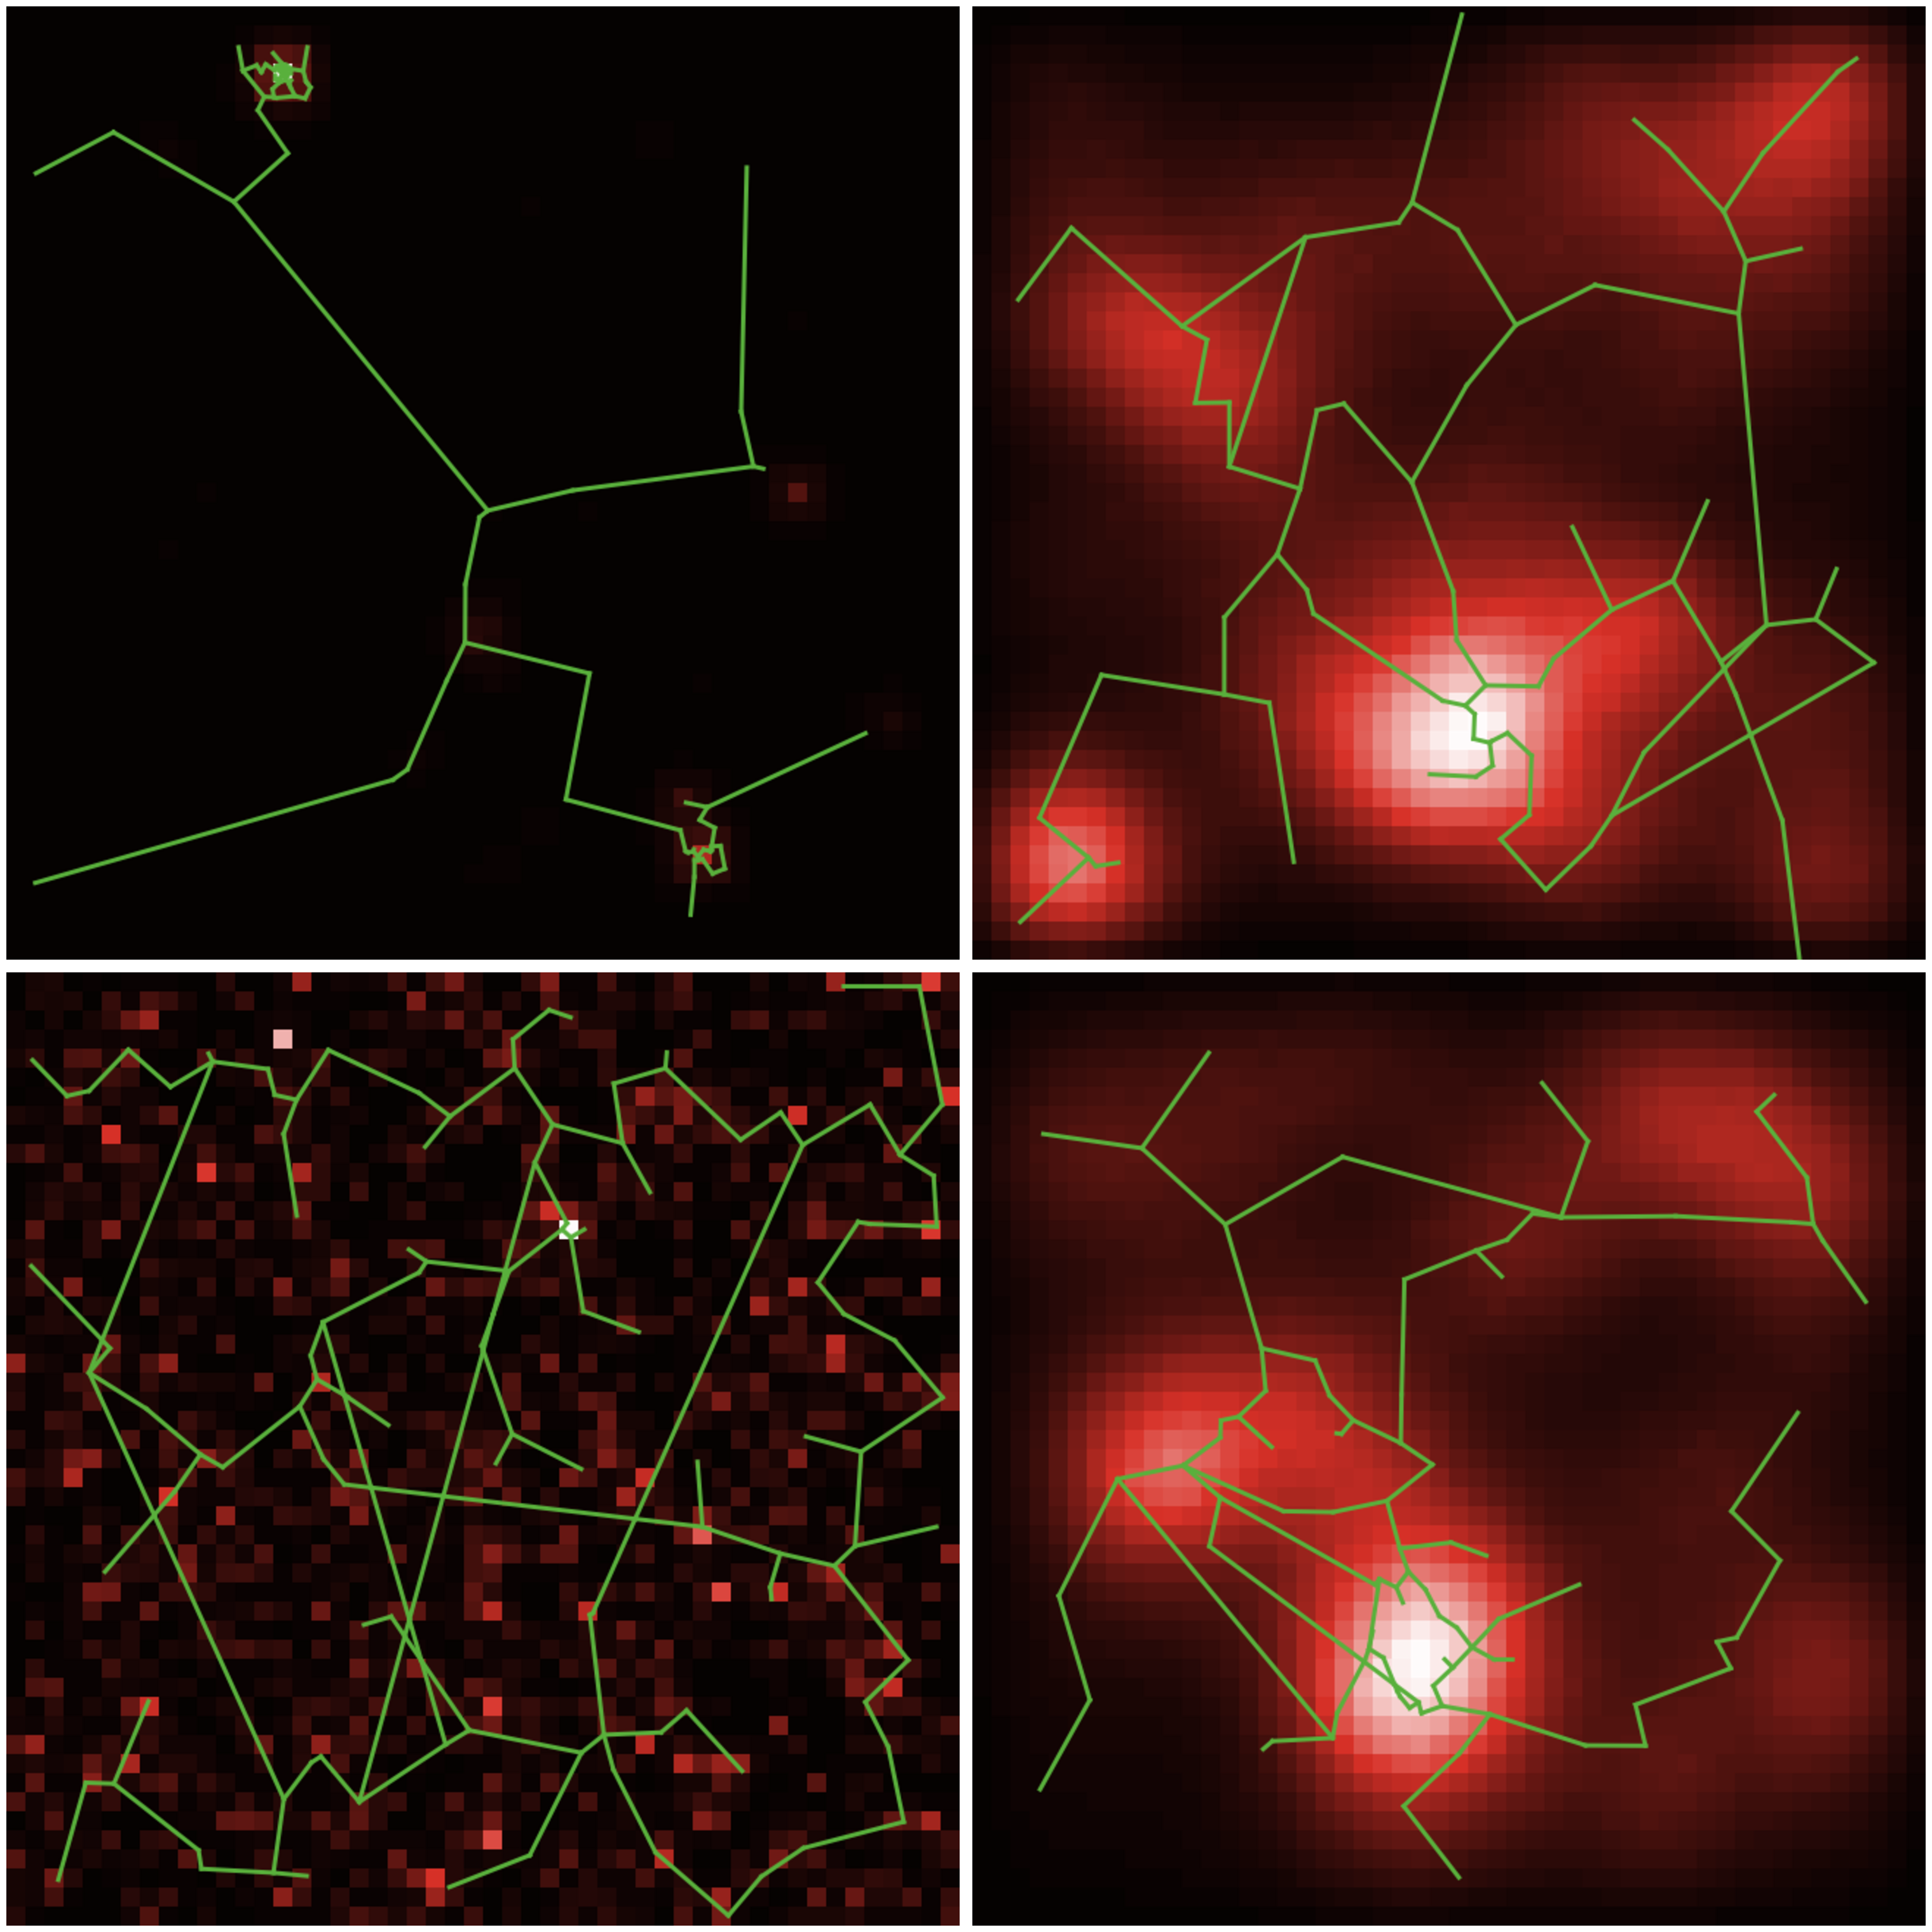
\includegraphics[width=\textwidth]{Figures/InteractionGibrat/Fig1}
\caption{\textbf{Time-series correlations as a function of distance.} Solid line correspond to smoothed correlations, computed between each pairs of normalized log-returns of population time-series, on successive periods given by curve color.}
\label{fig:interactiongibrat:ts-correlations}
\end{figure}
%%%%%%%%%%%%%%%%%%%%%%%%%





\paragraph{Model Exploration}{Exploration du modèle}


%\paragraph{Implementation}


Data preprocessing, result processing and models profiling are implemented in \texttt{R}. For performances reasons and an easier integration into the OpenMole software for model exploration~\citep{reuillon2013openmole}, a \texttt{scala} version was also developed. The question of trade-off between implementation performance and interoperability is a typical issue in this kind of model, as a fully blind exploration and calibration can be misleading for further research directions or thematic interpretations. A NetLogo implementation, allowing interactive exploration and dynamical visualization, was also developed for this reason. Source code for models, cleaned raw data, simulation data, and results used in this paper are available on the open repository of the project at \texttt{https://github.com/AnonymousAuthor1/InteractionGibrat.git}. We show in Figure~\ref{fig:interface} an example of model output. Cities color give city-level fit error and their size the population. Outliers can therefore easily be spotted (as Saint-Nazaire having the worst fit in the example shown) and possible regional effects identified. We illustrate in pink an example of geographical shortest path, from Rouen to Marseille, which reasonably corresponds to the actual current shortest path by highway. Top right plot shows trajectory in time for a given city, whereas the bottom right plot gives overall fit quality in time, by plotting simulated data against real data. The closest the curve is from the diagonal, the better the fit.


%%%%%%%%%%%%%%%%%%%
\begin{figure}
\centering
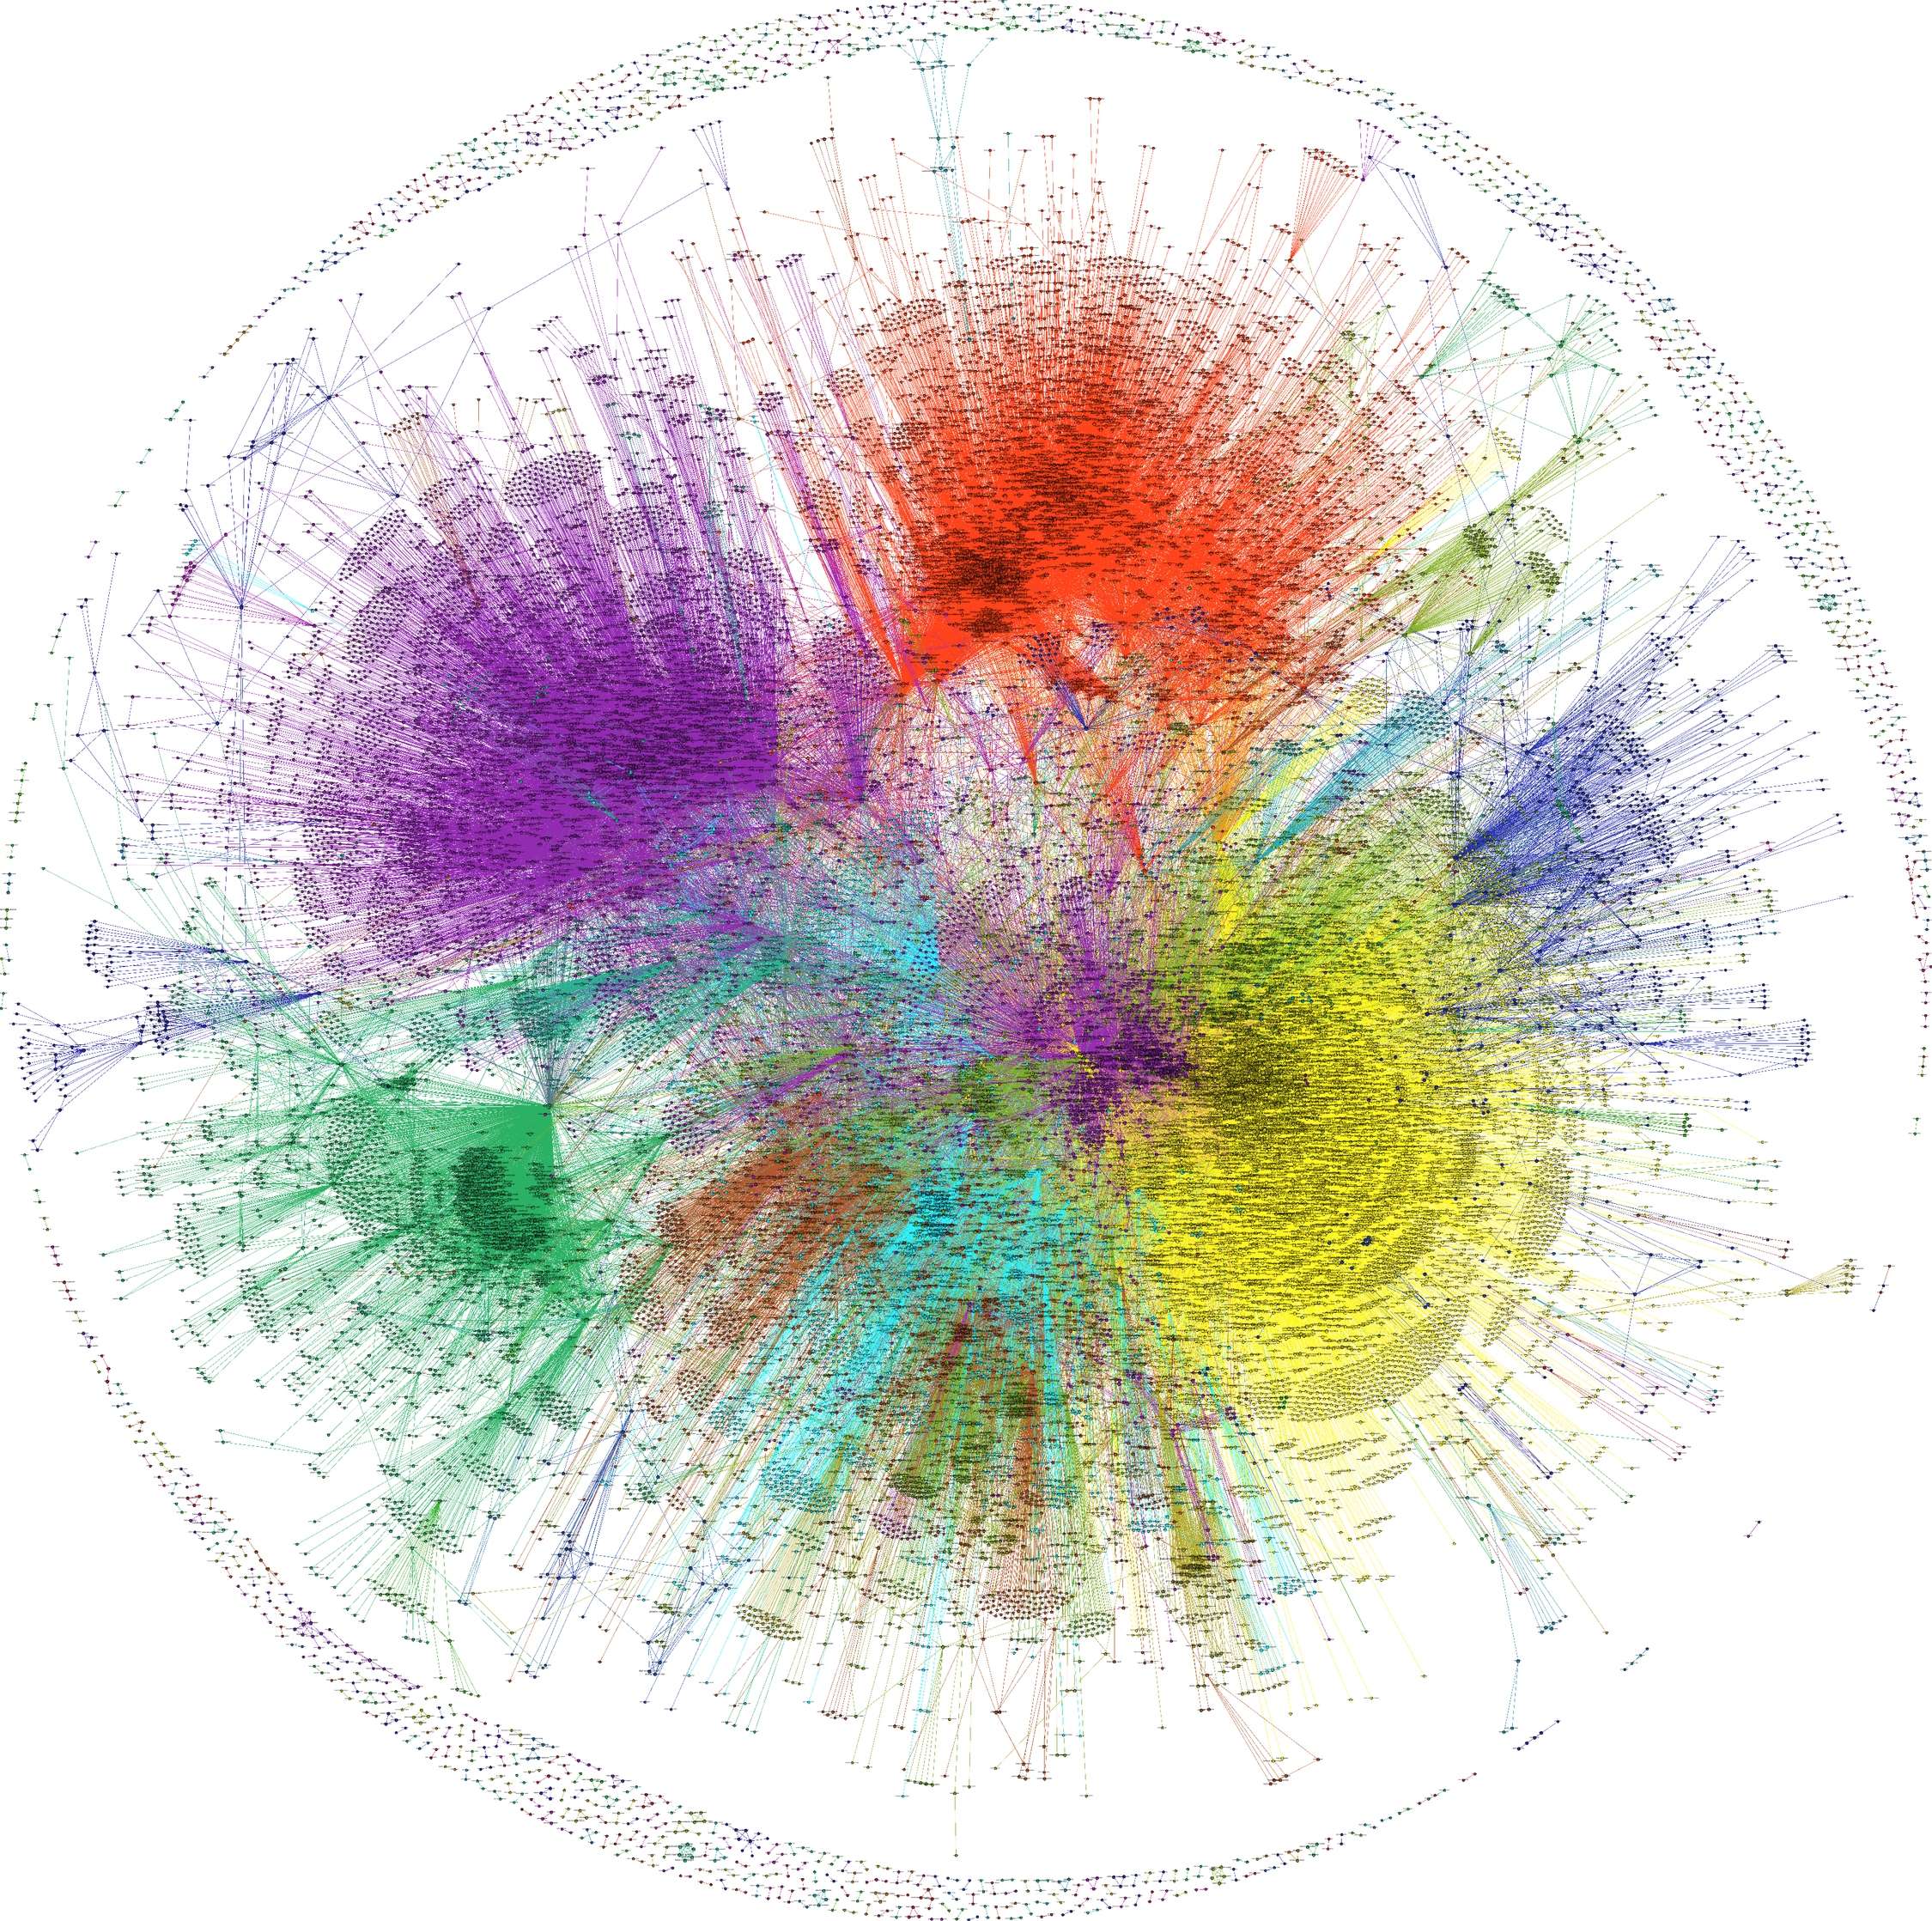
\includegraphics[width=\textwidth]{Figures/InteractionGibrat/Fig2}
\caption{Example of output of the model. The graphical interface allows to explore interactively on which cities changes operate after a parameter change, what is necessary to interpret raw calibration results.}
\label{fig:interactiongibrat:interface}
\end{figure}
%%%%%%%%%%%%%%%%%%%


%\paragraph{Behavior Patterns}

First model explorations, by simply sweeping fixed grids of the parameter space, already suggest the presence of network effects, in the sense that physical flow effectively have an influence on growth rates. We show in Figure~\ref{fig:networkeffects} a configuration of such a case. At fixed gravity parameters and growth rate, we study variations of the parameters $w_N, d_N$ and $\gamma_N$ and the corresponding response of $\varepsilon_G$ and $\varepsilon_L$. At fixed values of $\gamma_N$, we observe similar behaviors of the indicators when $w_N$ and $d_N$ change. The existence of a minimum of both as a function of $d_N$, that becomes stronger when $w_N$ increases, shows that introducing the network feedback terms improves local and global fits compared to the gravity model alone, i.e. that the associated process have potential explanatory power for growth patterns.


%%%%%%%%%%%%%%%%%%%%
\begin{figure}
\centering
\includegraphics[width=\textwidth]{figures/Fig3}
\caption{Evidence of network effects revealed by model exploration. Left plot gives $\varepsilon_G$ as a function of $d_N$ for varying $r_0/w_N$, at fixed gravity effect and $\gamma_N=3$. Right plot is similar for $\varepsilon_L$}
\label{fig:networkeffects}
\end{figure}
%%%%%%%%%%%%%%%%%%%%



























\subsection{Discussion}{Discussion}

